\documentclass[10pt]{article}
\usepackage[margin=0.7in]{geometry}
\usepackage{amsmath, amssymb}
\usepackage{graphicx}
\usepackage{booktabs}
\usepackage[font=small, labelfont=bf]{caption}
\usepackage{subcaption}
\usepackage{float}
\usepackage[hidelinks]{hyperref}
\setlength{\parskip}{3pt}
\setlength{\parindent}{0pt}
\setlength{\abovedisplayskip}{3pt}
\setlength{\belowdisplayskip}{3pt}

\title{\vspace{-1.6cm}MATH550 HW1}
\author{Naima Shariff}
\date{}

\begin{document}
\maketitle
\vspace{-1.4cm}

\section*{Problem 1}

We solve the steady Stokes equations $\mu\nabla^2\mathbf{u} - \nabla P = \mathbf{f}$, $\nabla\cdot\mathbf{u} = 0$ with $\mu = 1$ on the unit square, periodic in $x$, with $U = 0$ and $V = -3.5$ on the walls $y = 0, 1$. The equations are discretized on a staggered (MAC) grid: $P$ at cell centers, $U$ on vertical faces with ghost rows outside the walls, and $V$ on horizontal faces including the walls. All derivatives are second-order centered differences. The unknowns $[U, V, P]$ are assembled into a single sparse system $A\mathbf{x} = \mathbf{b}$ and solved with a sparse direct solver. Pressure is pinned to zero in one cell to remove its free constant. The code is verified against the manufactured solution
\[
U = \sin(2\pi y)\sin(2\pi x), \quad V = -3.5 + \cos(2\pi x)\,(\cos(2\pi y) - 1), \quad P = \sin(2\pi y)\cos(2\pi x),
\]
with $f$ and $g$ obtained by substituting these fields into the momentum equations. At $N = 64$ the numerical and analytical fields are indistinguishable (Figs.~\ref{fig:speed}, \ref{fig:pressure}). The maximum speed error is $1.6\times10^{-3}$ on a speed of order 5, and the maximum pressure error is $4\times10^{-4}$ on a pressure of order 1. Both errors are smooth and follow the structure of the solution.

Note: No boundary conditions are imposed on $P$. Pressure acts as the Lagrange multiplier that enforces $\nabla\cdot\mathbf{u} = 0$, and is determined by the velocity boundary conditions up to an additive constant. 

\begin{figure}[H]
\centering
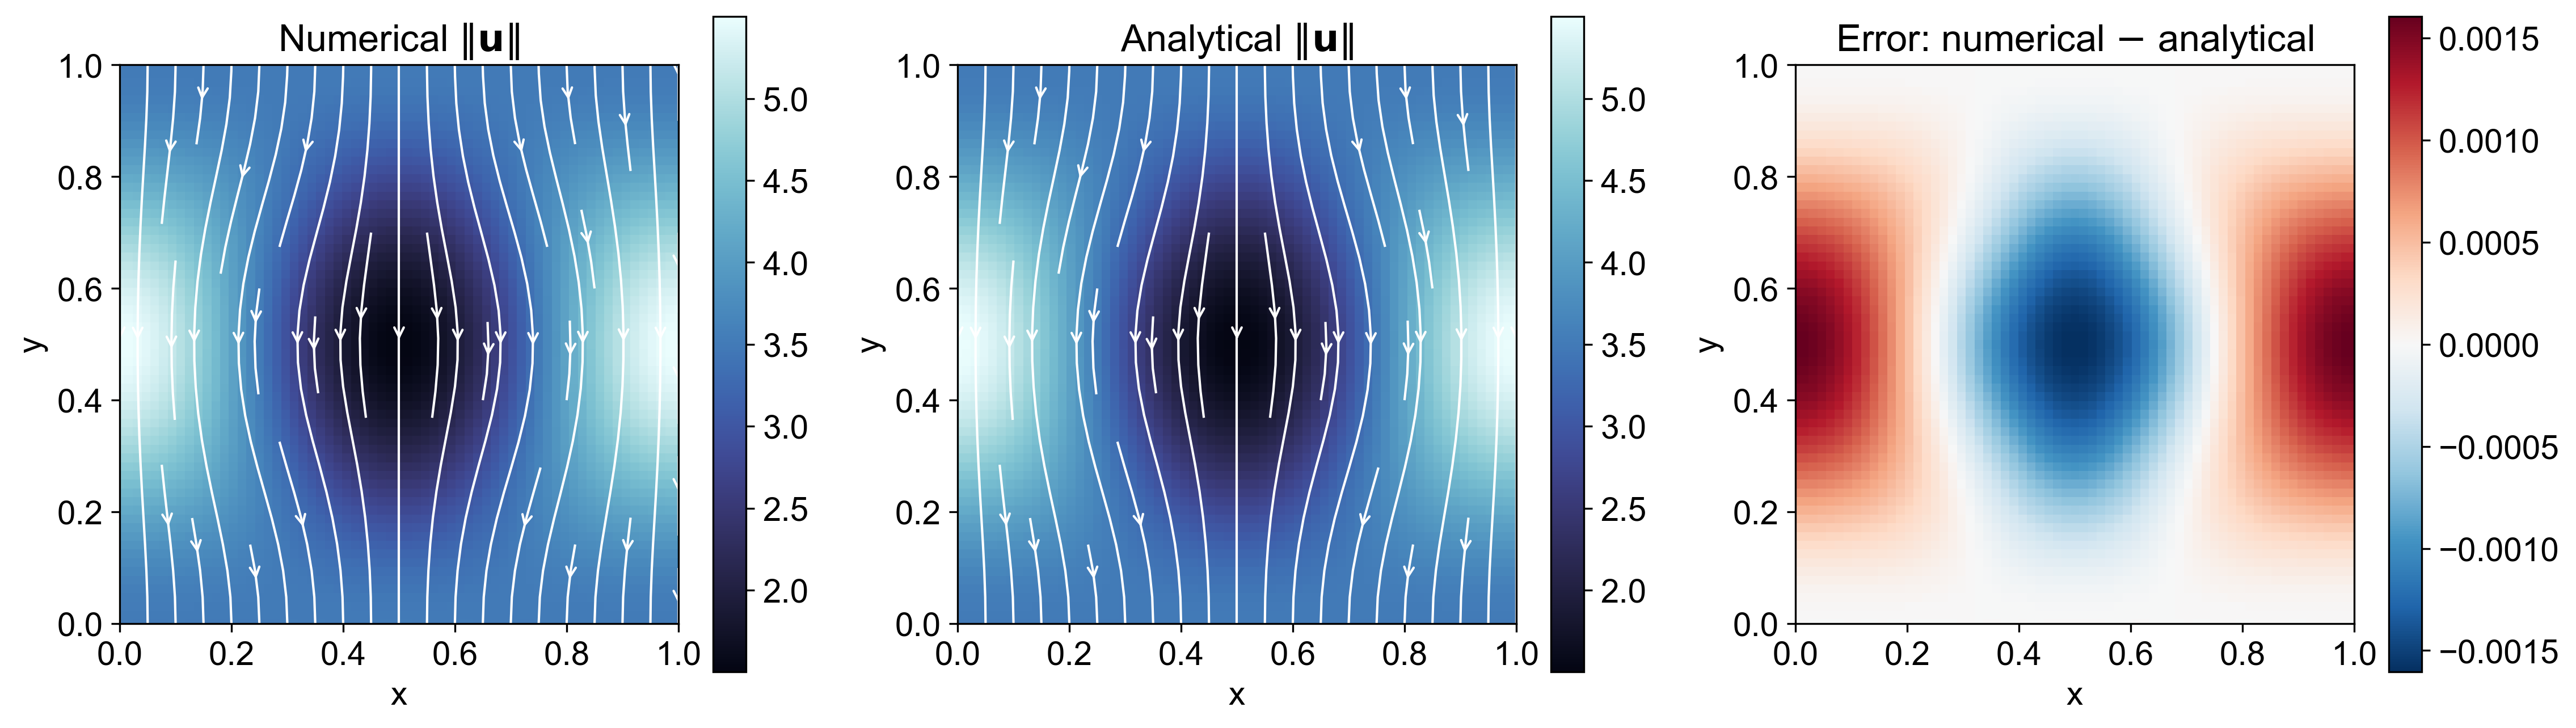
\includegraphics[width=0.9\textwidth]{fig1_umag.png}
\caption{Speed $\|\mathbf{u}\|$ with streamlines at $N = 64$: numerical (left), analytical (center) and their difference (right). Velocities are averaged from the faces to the cell corners for plotting.}
\label{fig:speed}
\end{figure}

\begin{figure}[H]
\centering
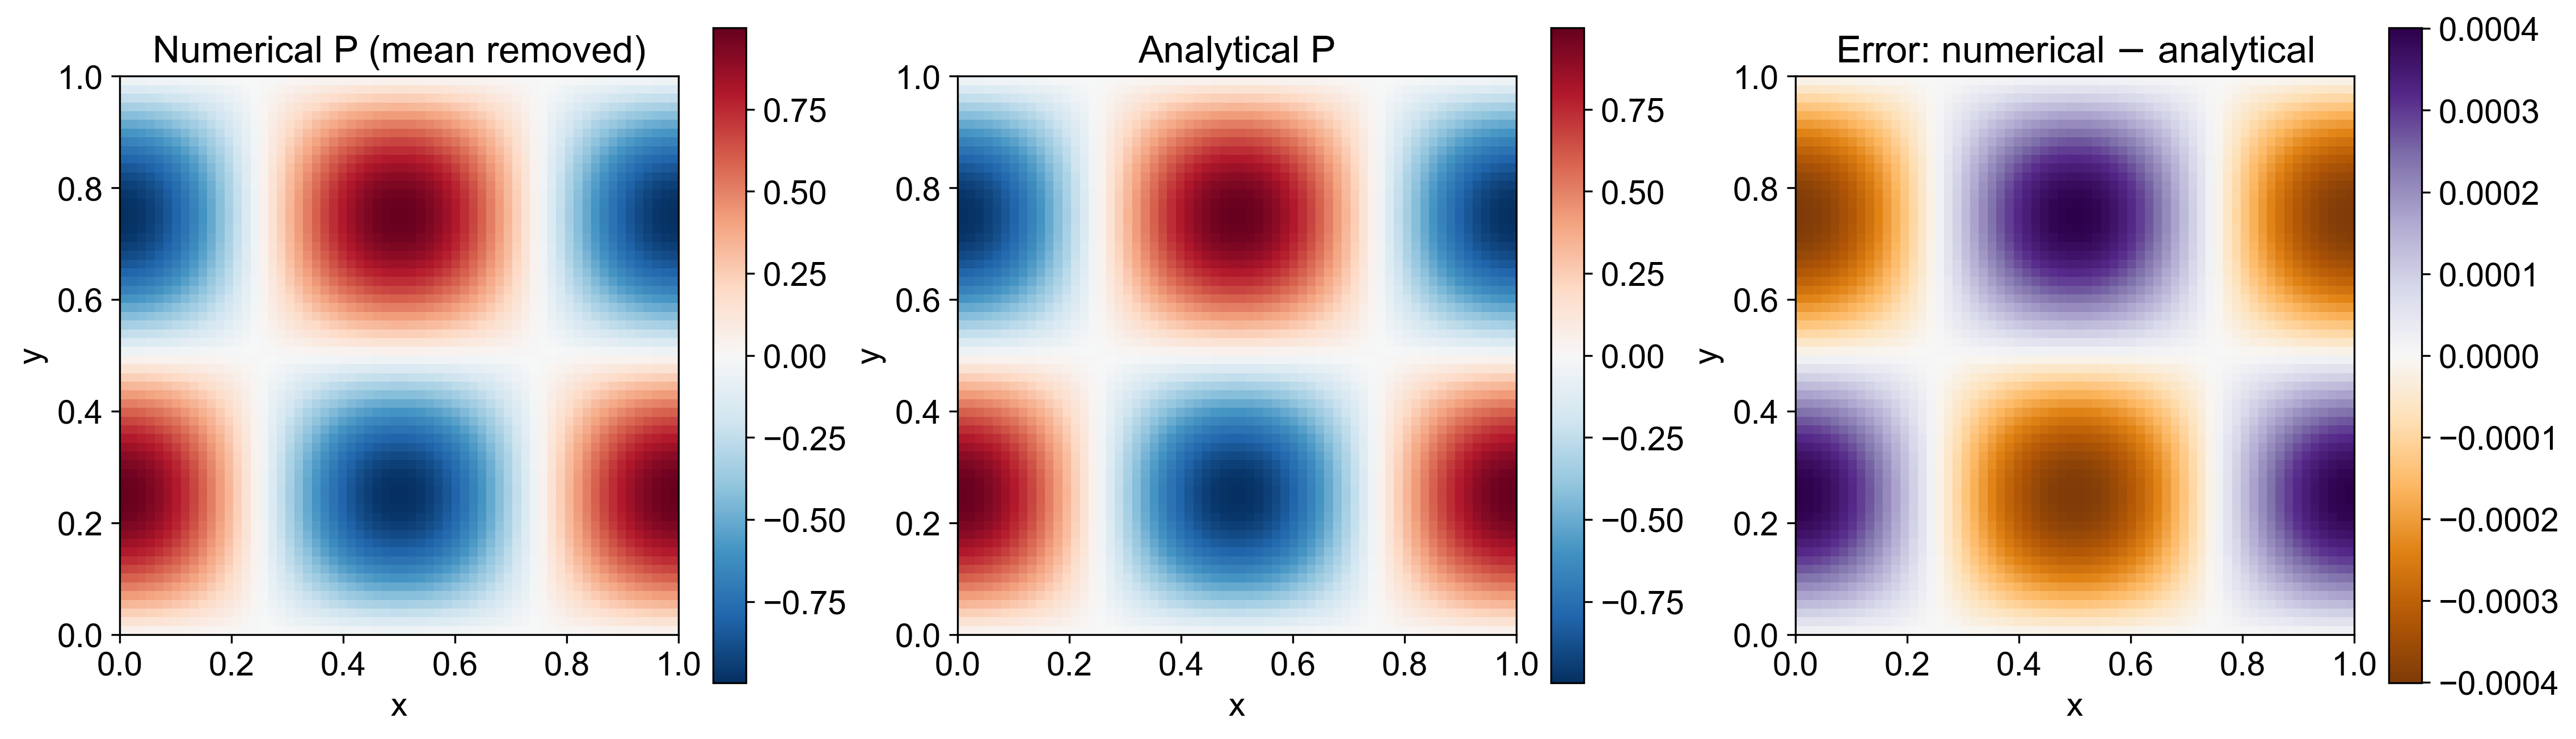
\includegraphics[width=0.9\textwidth]{fig2_pressure.png}
\caption{Pressure at $N = 64$, mean removed: numerical (left), analytical (center) and their difference (right). The mean is removed from both fields because the numerical pressure is pinned in one cell and is defined only up to a constant.}
\label{fig:pressure}
\end{figure}

\section*{Problem 2: Error Analysis}

The relative $L_2$ error $\|X_{\text{num}} - X_{\text{an}}\|_2 / \|X_{\text{an}}\|_2$ is computed for $X = U, V, P$ at the grid locations where each field is stored, with the ghost rows of $U$ excluded and the mean removed from $P$. Over $N = 10$ to $100$, the fitted slopes are $-2.01$ for $U$, $-1.99$ for $V$ and $-2.00$ for $P$. All three error curves are parallel to the second-order reference line (Fig.~\ref{fig:conv}).

\begin{figure}[H]
\centering
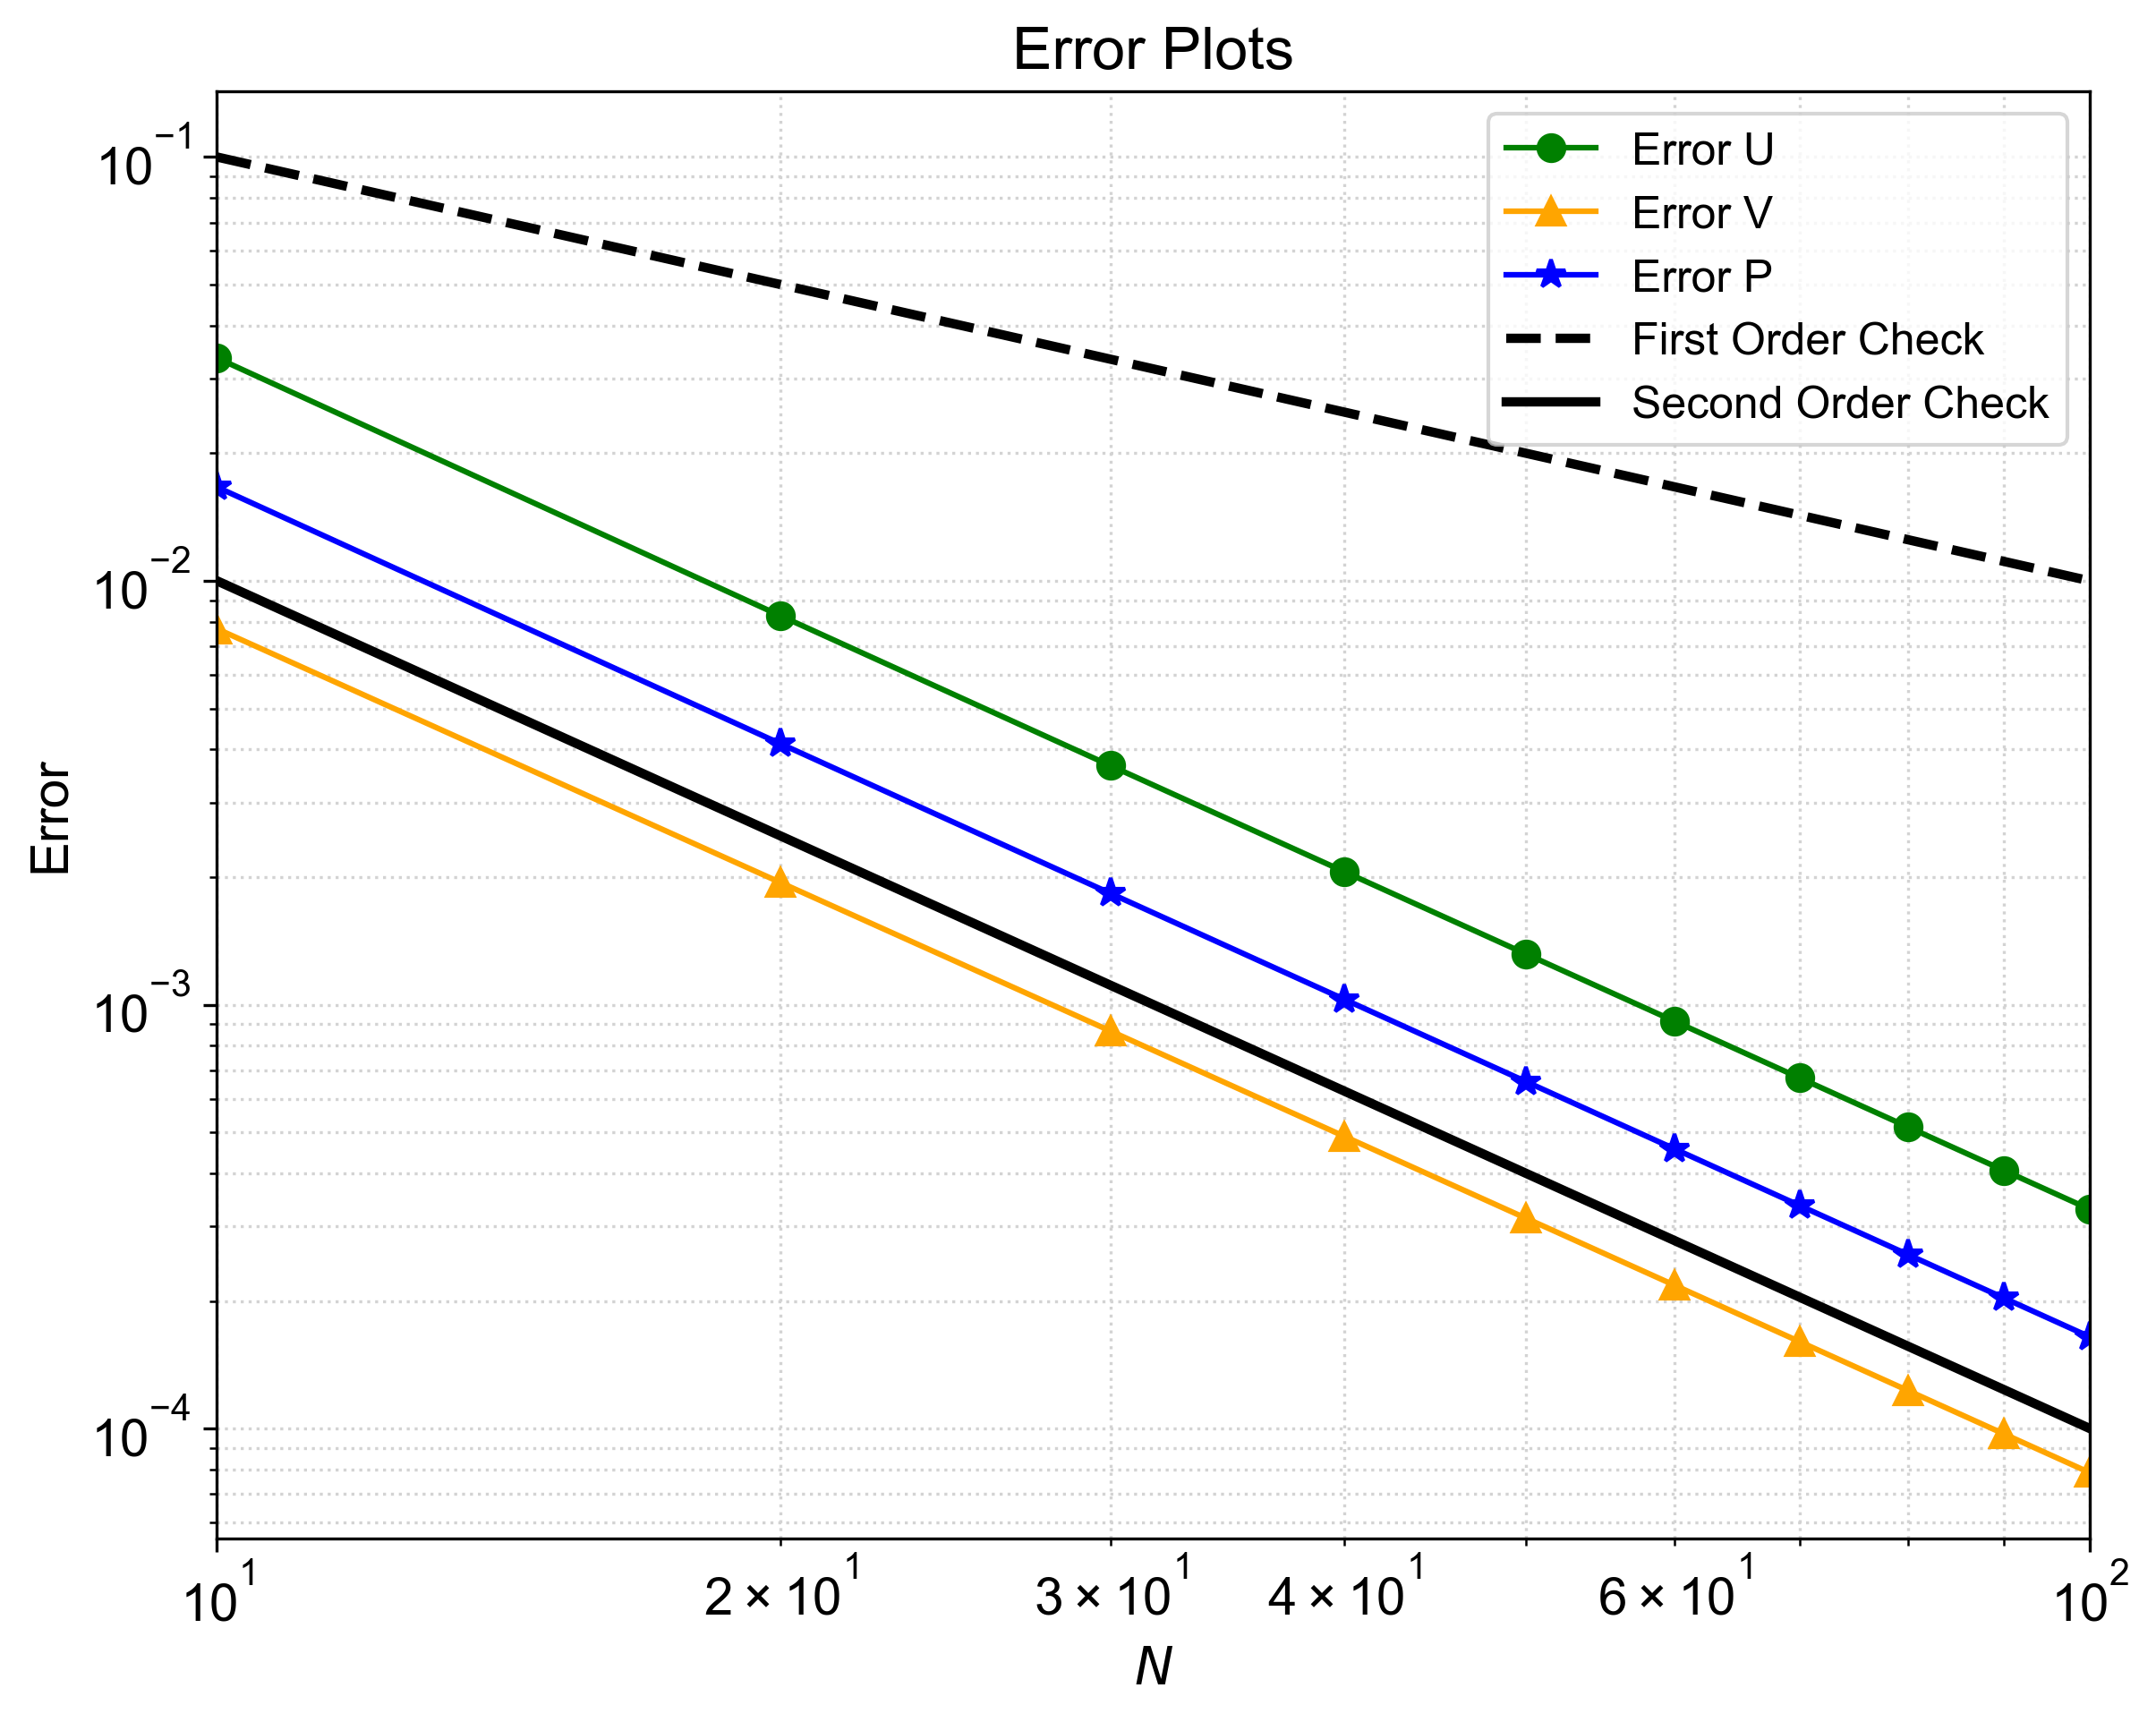
\includegraphics[height=8cm]{fig3_convergence.png}
\caption{Relative $L_2$ error of $U$, $V$ and $P$ against $N$, with first-order ($1/N$) and second-order ($1/N^2$) reference lines. All three errors decrease at second order.}
\label{fig:conv}
\end{figure}

 
\section*{Problem 3: Charlie's Rule}

Two extensions of the solver are explored: a timing comparison between the sparse direct solver and GMRES, and Stokes-Darcy flow through a porous medium with four impermeable grains.

\textbf{Direct solver against GMRES.} 

The sparse direct solve was timed against restarted GMRES without a preconditioner, both on the assembled matrix and on a \texttt{LinearOperator} that supplies only the product $A\mathbf{v}$. The GMRES tolerance was set to $0.1h^2$, the level of the discretization error. With a restart length of 200, GMRES converges at every grid size and stays within a factor of about 1.5 of the direct solver (Table~\ref{tab:timing}). The restart length is decisive. With a restart length of 20, GMRES needed over 22\,000 iterations at $N = 32$ and did not converge within 40\,000 iterations at $N = 64$, because each restart discards the Krylov basis before the solution is resolved.
 
\begin{table}[H]
\centering
\small
\begin{tabular}{rrrrrc}
\toprule
$N$ & Unknowns & Direct (s) & GMRES, matrix (s) & GMRES, operator (s) & Converged \\
\midrule
16 & 816     & 0.0026 & 0.0035 & 0.0027 & yes \\
32 & 3\,168  & 0.0146 & 0.0207 & 0.0201 & yes \\
64 & 12\,480 & 0.1465 & 0.2267 & 0.2206 & yes \\
\bottomrule
\end{tabular}
\caption{Solve times for the sparse direct solver and GMRES(200) without a preconditioner, tolerance $0.1h^2$, maximum 300 restart cycles. Matrix assembly is excluded from the timings.}
\label{tab:timing}
\end{table}
 
\noindent\begin{minipage}[c]{0.56\textwidth}
\textbf{Stokes-Darcy flow through grains.} 

A drag term is added to the momentum equations, giving the Brinkman equations
\[
\mu\nabla^2\mathbf{u} - \alpha(x, y)\,\mathbf{u} - \nabla P = 0, \qquad \nabla\cdot\mathbf{u} = 0, \qquad \alpha = \mu/\kappa,
\]
where $\kappa$ is the permeability. In open fluid $\alpha = 0$ and the Stokes equations are recovered. Inside a grain $\alpha$ is large and the balance approaches Darcy's law, $\mathbf{u} \approx -(\kappa/\mu)\nabla P$. In the discretization this changes only the diagonal of the interior momentum rows, from $-4\mu/h^2$ to $-4\mu/h^2 - \alpha$. The continuity rows are unchanged, and the maximum discrete divergence is $2\times10^{-7}$. Four grains of radius 0.15 are placed one per quadrant, with $\alpha = 10^6$ inside (well above $\mu/h^2 \approx 1.6\times10^4$ at $N = 128$, so the grains are effectively impermeable) and a smooth $\tanh$ transition at the edge. The source terms are set to zero, so the flow is driven only by the wall velocity. The flow divides around the grains and accelerates through the gaps at $x = 0$ and $x = 0.5$, which carry the full flux through 40\% of the width (Fig.~\ref{fig:grains}).
\end{minipage}\hfill
\begin{minipage}[c]{0.41\textwidth}
\centering
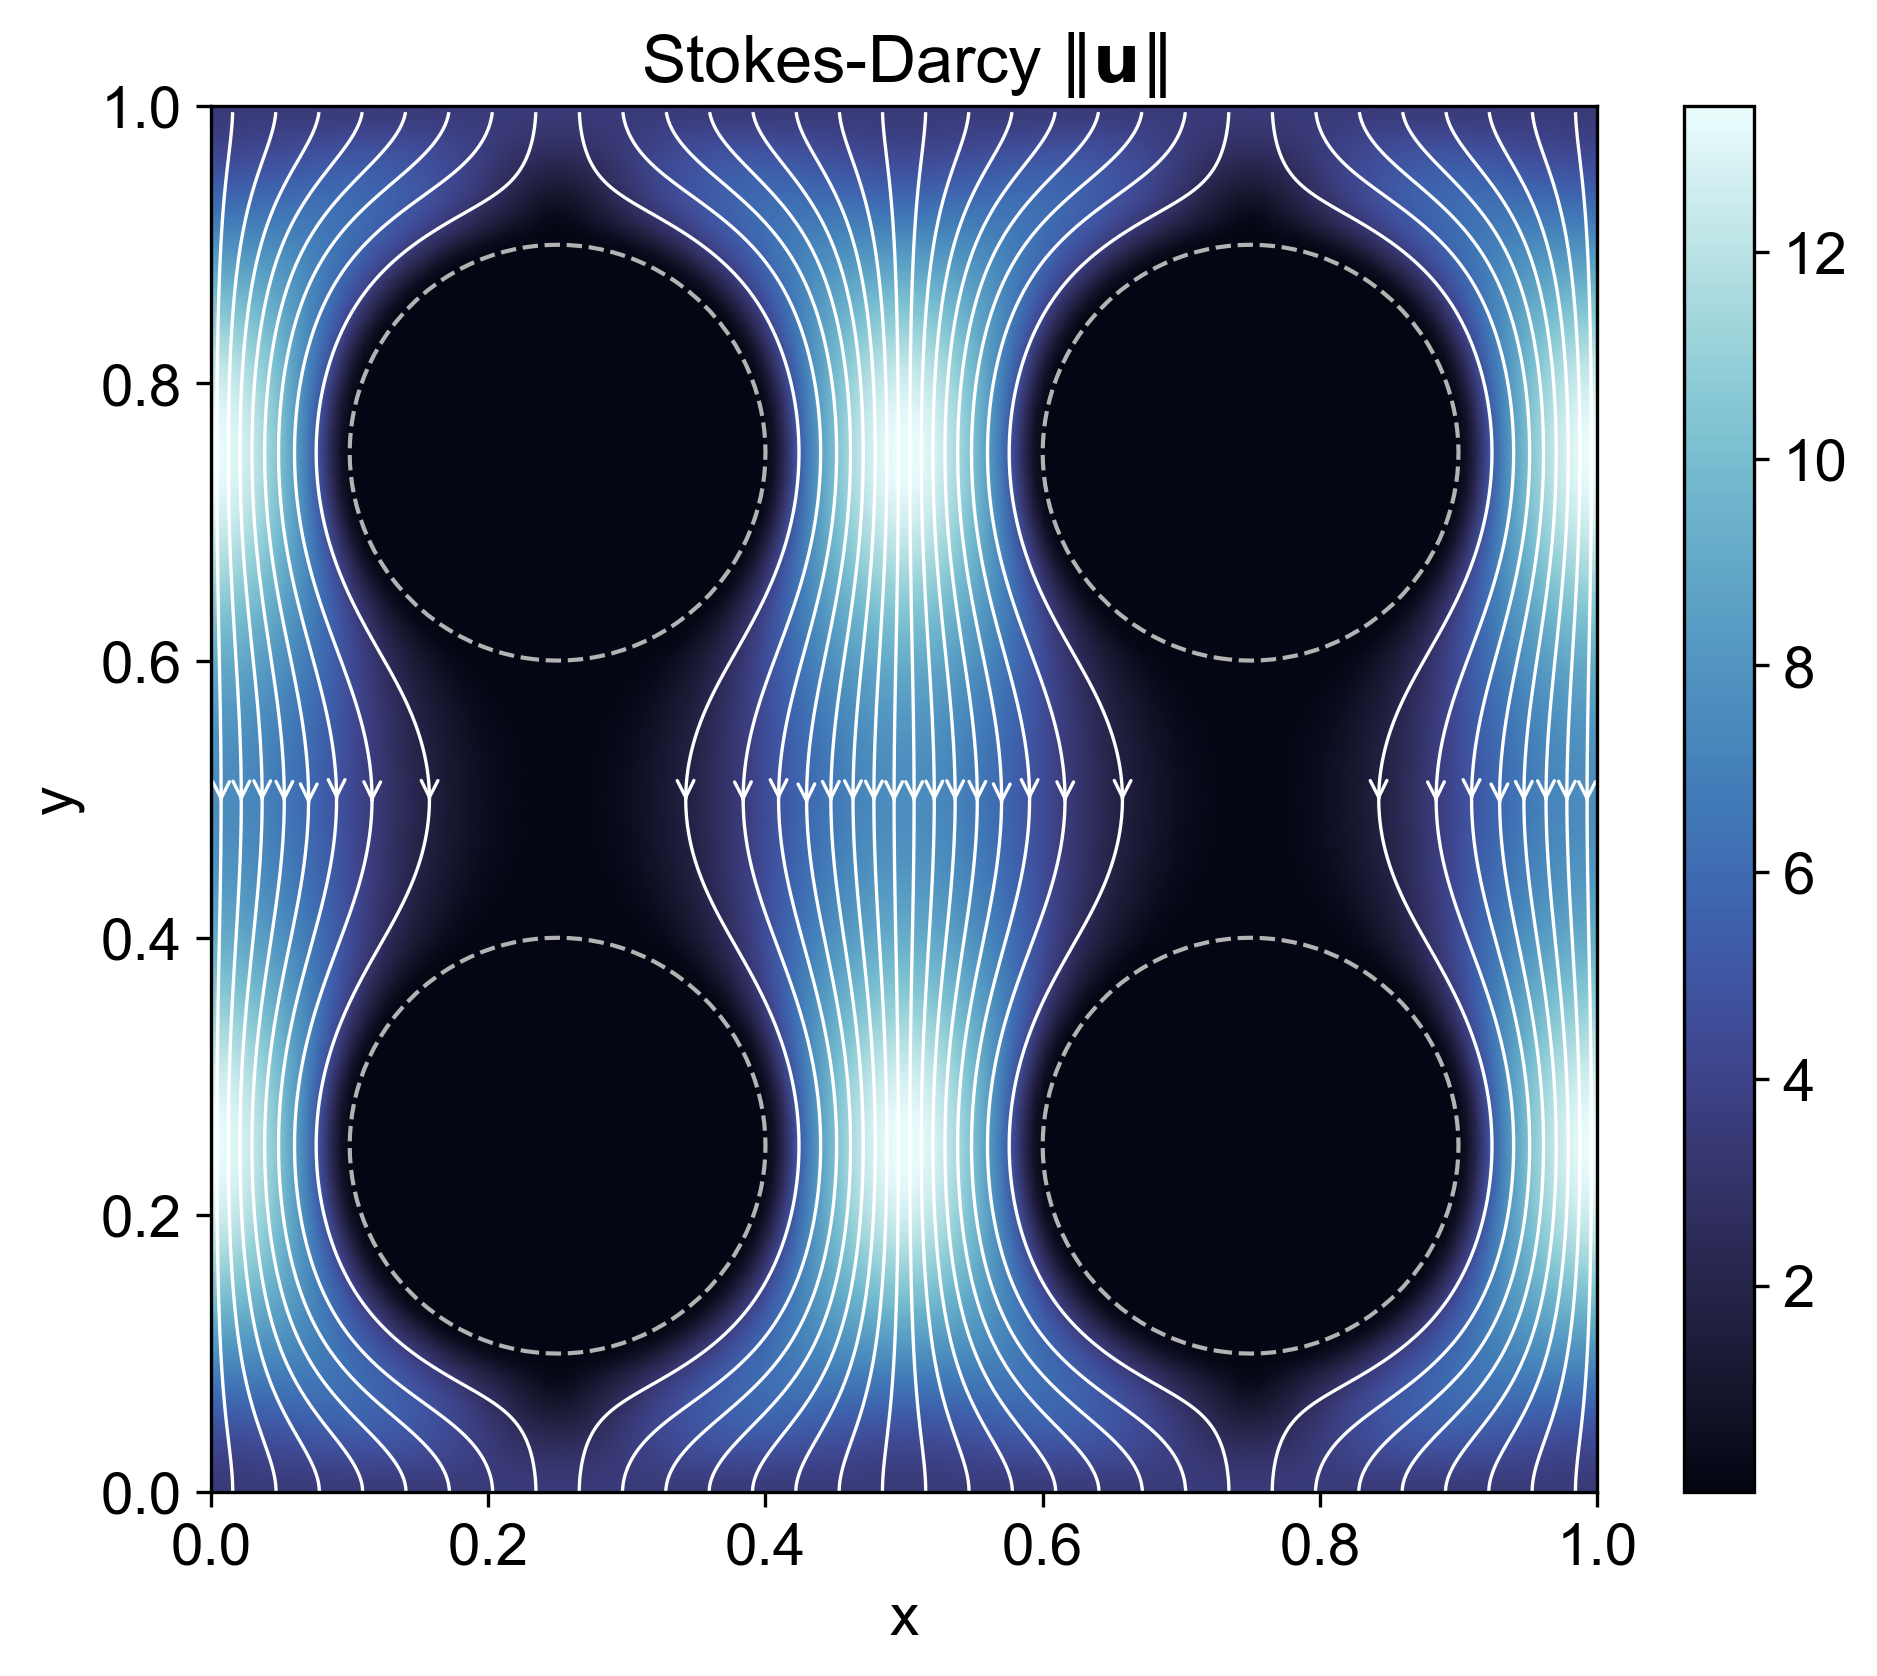
\includegraphics[width=\textwidth]{fig4_darcy.png}
\captionof{figure}{Stokes-Darcy speed and streamlines at $N = 128$ with four impermeable grains (dashed outlines), $\alpha = 10^6$ inside the grains and $f = g = 0$. Streamlines are seeded along the top wall.}
\label{fig:grains}
\end{minipage}


All code, figures and the notebook used to produce this report are available in the GitHub repository \url{https://github.com/naimash/MATH550_HW}.

\vspace{-4pt}
{\footnotesize\textit{Acknowledgement: The Stokes-Darcy extension in Problem 3 was developed with assistance from an AI model (Claude, Anthropic, Model: Sonnet).}}
 
\end{document}
